\documentclass{CBM-PR-2020}
\usepackage{graphicx}
\usepackage[utf8]{inputenc}
\usepackage{amsmath}
\usepackage{amssymb}
\setlength{\titleblockheight}{35mm}

\begin{document}
\title{
The first mPSD beam test results at mCBM in 2020
%\thanks{
%Work supported by XXX (Exchange XXX with your grant).
%}
}

\author[a]{D. Finogeev}


\affil[a]{Institute for Nuclear Research RAS, Moscow, Russia,}



%\author[1]{D. Finogeev, F. Guber, N. Karpushkin, A. Makhnev, S. Morozov, D. Serebryakov}
%\affil[1]{INR RAS, Moscow, Russia}

\maketitle


At the end of 2019 and beginning of 2020, beam tests at mCBM@SIS18 were carried out with Au and Pb ions at 1.01 - 1.22 AGeV energy range. Test of the mPSD prototype as a part of mCBM experiment allows to approve and verify the feasibility of the PSD readout concept. The prototype includes crucial parts of the readout such as Addon prototype board and ADC FPGA readout board. In this setup, Addon incorporated only the single-ended to differential converters and the necessary power systems. Photo of the assembled FEE setup is represented on figure~\ref{fig:4}.

\begin{figure}[htbp]
\centering % \begin{center}/\end{center} takes some additional vertical space
\raisebox{-0.5\height}{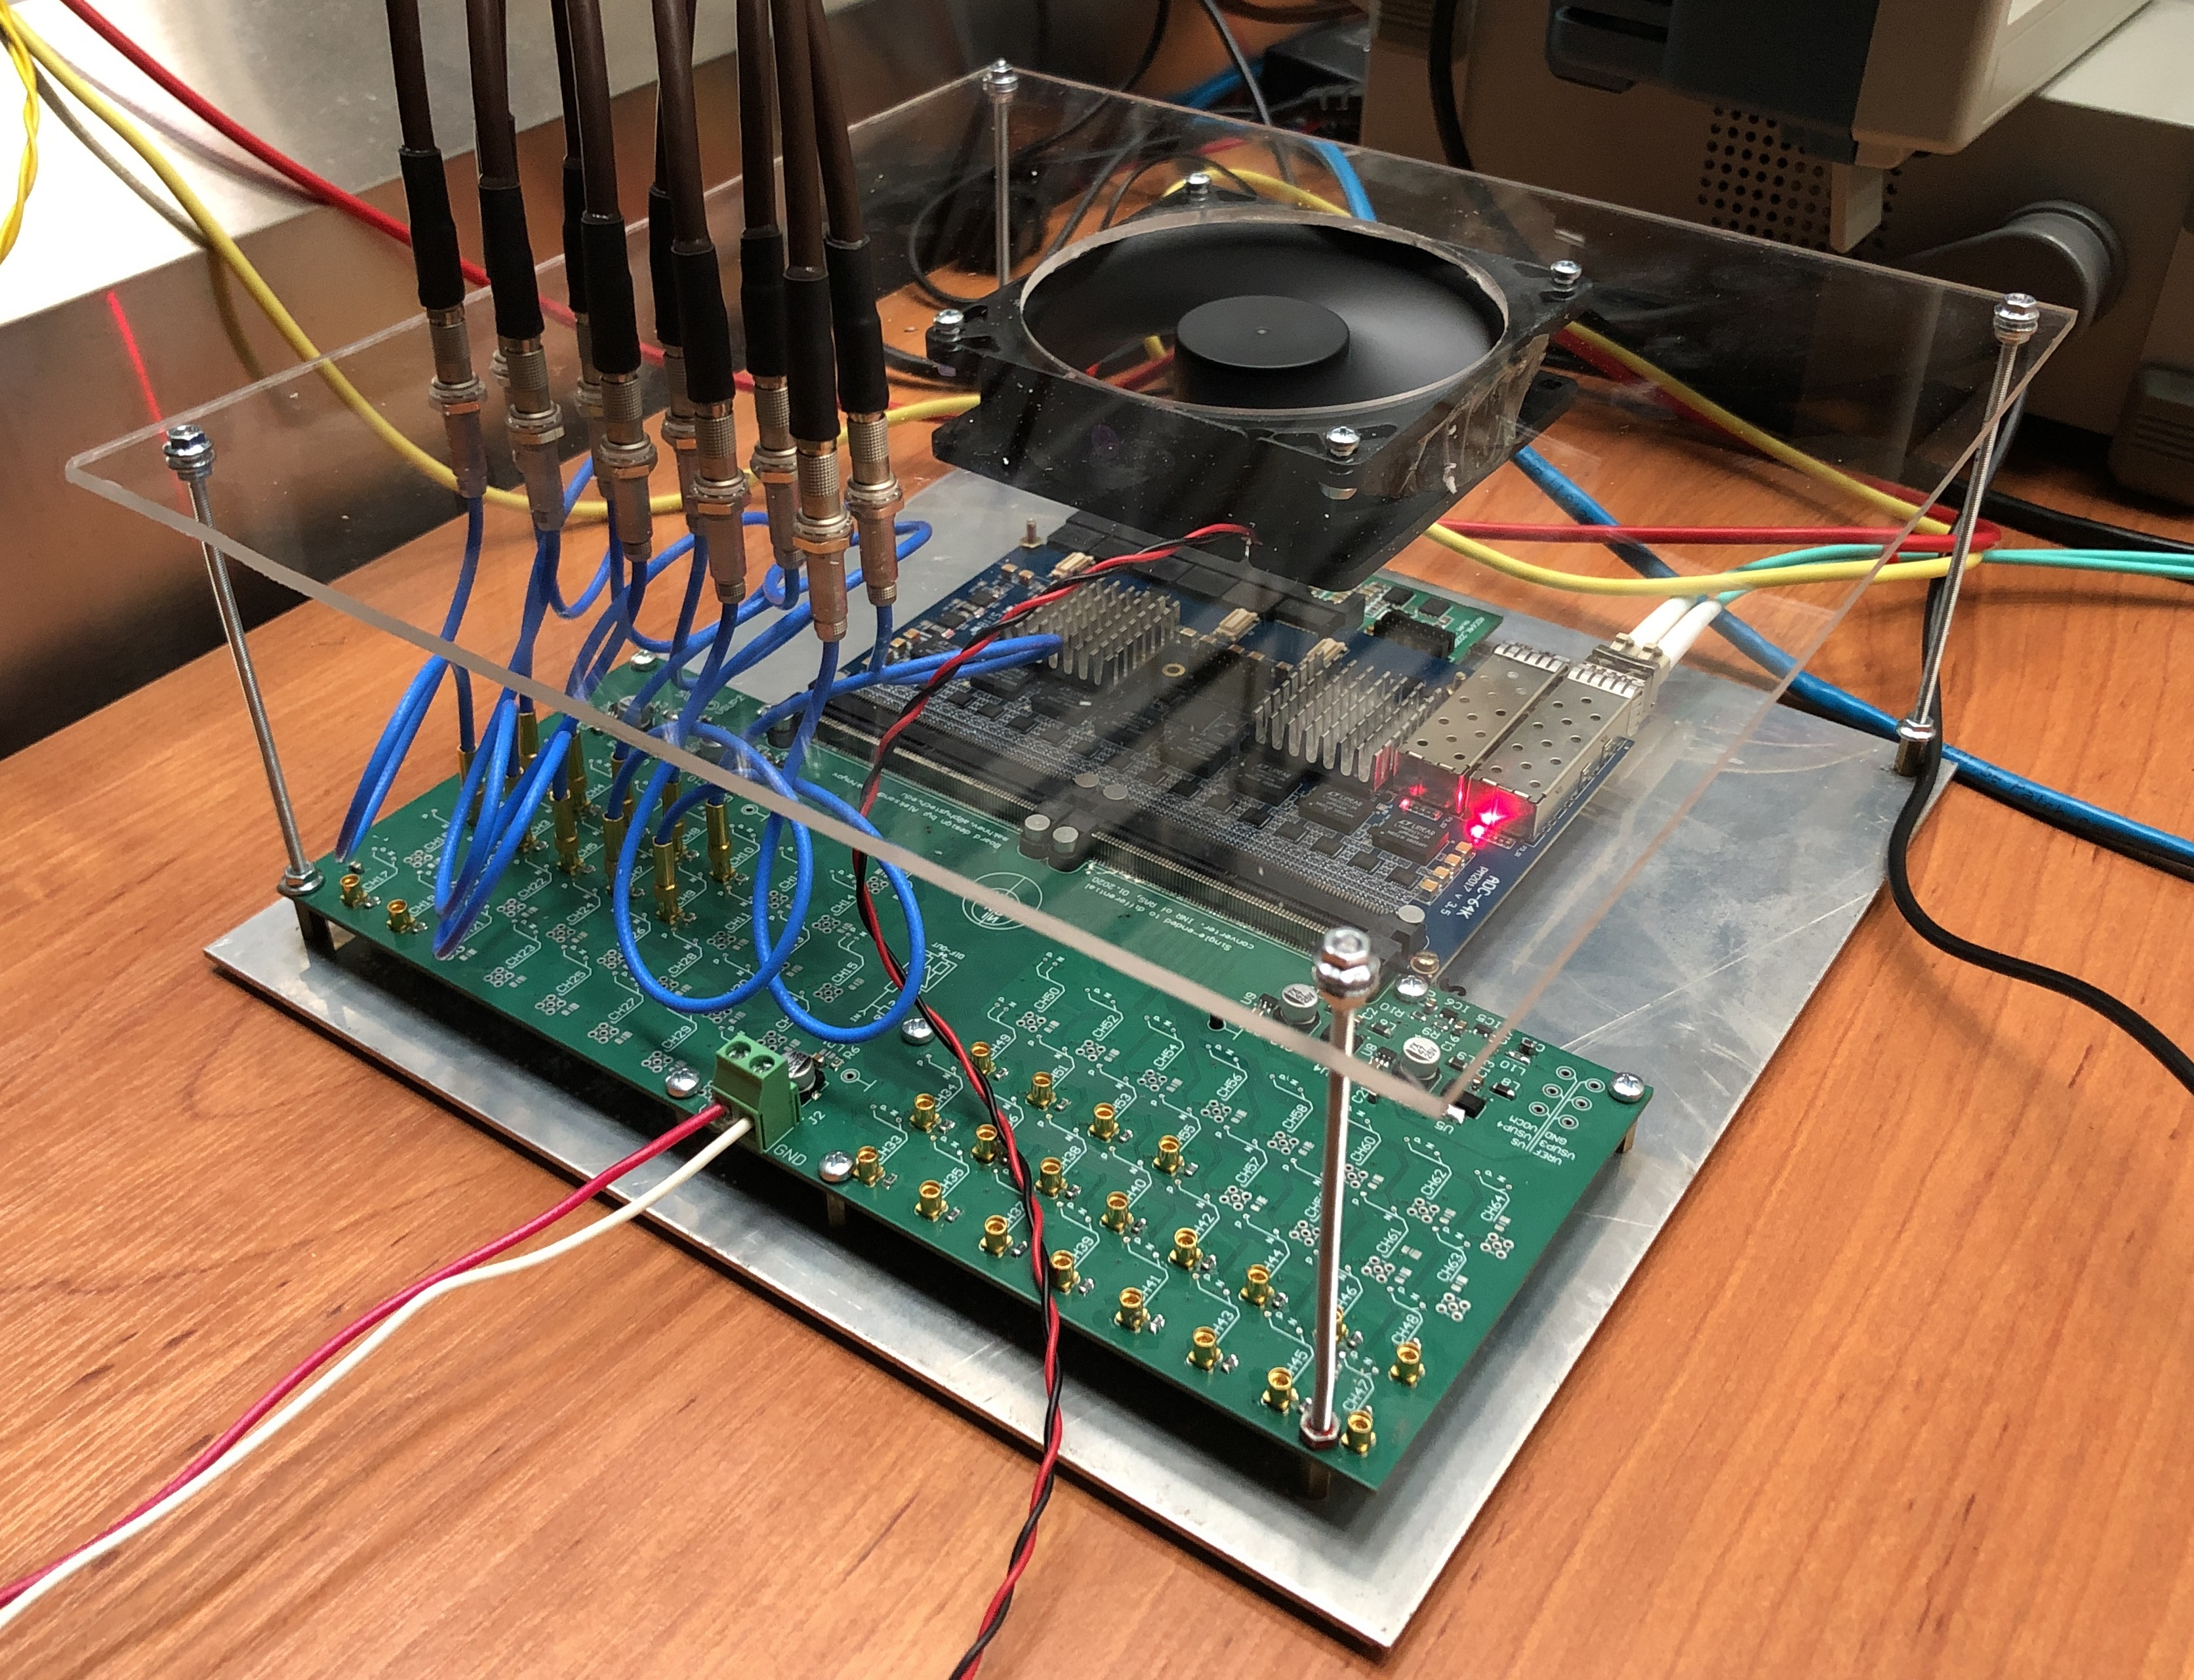
\includegraphics[width=.2\textwidth]{mPSD_FEE_photo.JPG}}
\qquad
\raisebox{-0.5\height}{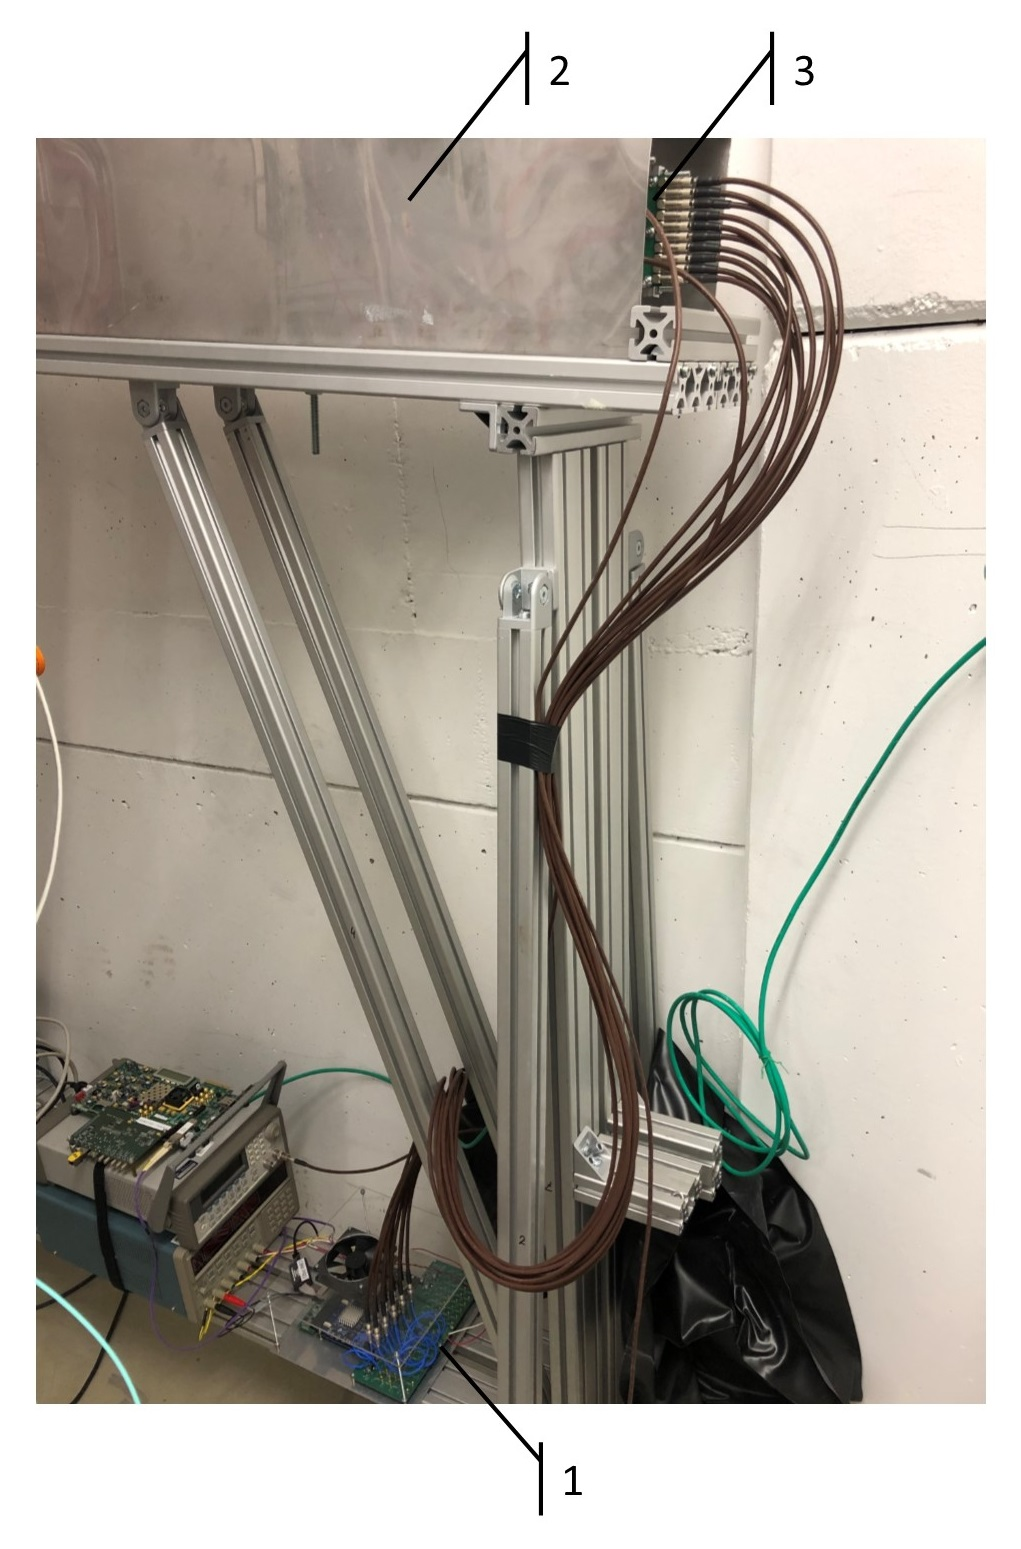
\includegraphics[width=.2\textwidth]{mPSD_module_photo.JPG}}
\caption{\label{fig:4} Photo of the ADC board assembled with the Addon board prototype (left); photo of mPSD module connected to FEE (right; 1 - Addon and ADC assembly, 2 - mPSD, 3 - MPPC board)}
\end{figure}

ADC FPGA board was connected to mCBM DAQ via GBT protocol used for data transport, clock distribution and configuration purposes. ADC was used in 80 Msps digitization mode. Each channel is triggered independently by amplitude threshold crossing and extracts data points from the waveform of the input signal measured in a fixed gate. ADC takes data in trigger-less readout mode according to CBM DAQ requirements. In addition, prototypes of all crucial software parts such as data unpacker, event building and data monitor were developed and tested.


One of the prime aims of mCBM is to test and validate the data processing concept and the reconstruction software which are being developed for the full CBM experiment. mCBM thus will be a demonstrator for the computing concept of CBM, including the reconstruction of events and selection of data in real-time and the full offline data analysis. It is thus planned to use already existing software components as far as possible for both online and offline computing in mCBM.
The challenge of the trigger-less readout is time synchronization and event building procedure. It is necessary to construct events from signals based on their time stamps while data processing.

\begin{figure}[htbp]
\centering % \begin{center}/\end{center} takes some additional vertical space
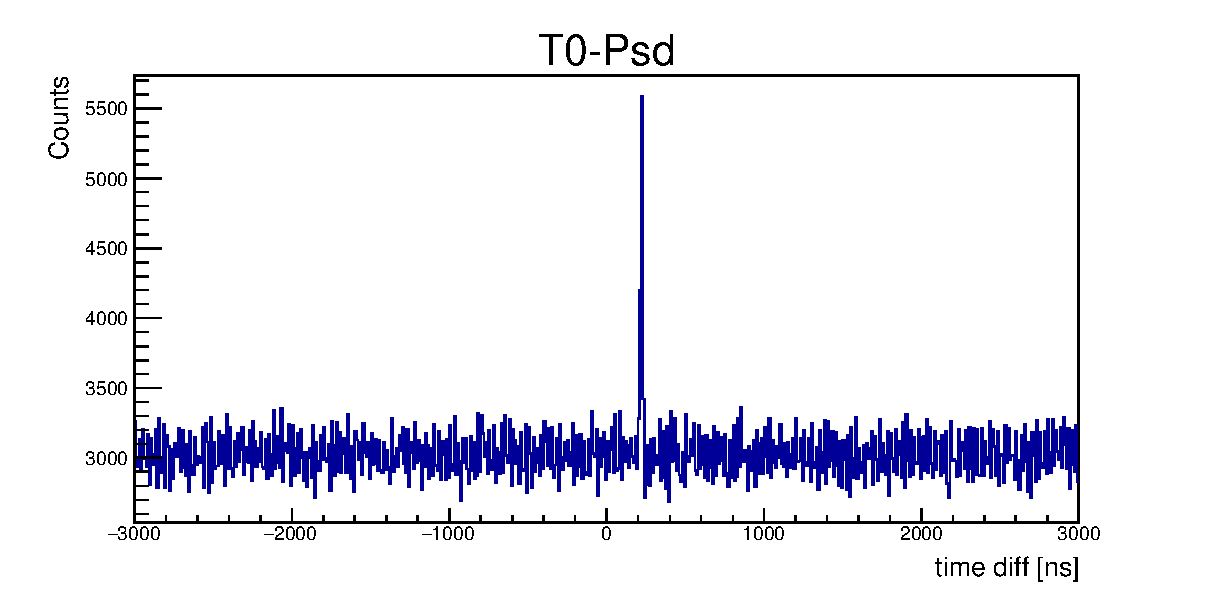
\includegraphics[width=.5\textwidth]{582_time_spectrum.eps}
\quad
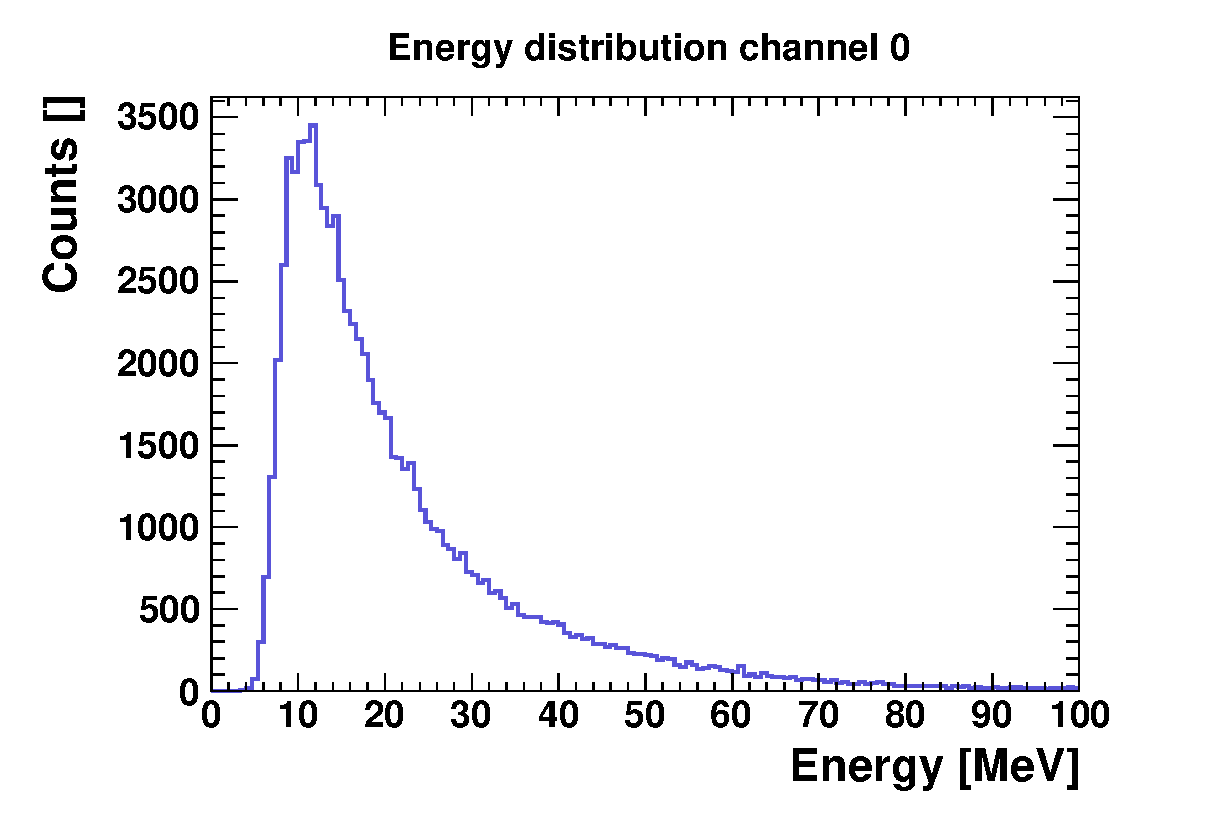
\includegraphics[width=.35\textwidth]{en_distrib_ch0.eps}
\caption{\label{fig:6} T0-Psd time correlation(left);  mPSD energy deposition in first section (right)}
\end{figure}




\begin{thebibliography}{9}   % Use for  1-9  references
\bibitem{1}
  D.~Finogeev, F.~Guber, N.~Karpushkin, A.~Makhnev, S.~Morozov and D.~Serebryakov,
  ``Development of readout chain for CBM Projectile Spectator Detector at FAIR,''
  J.\ Phys.\ Conf.\ Ser.\  {\bf 1690} (2020) no.1,  012059.
  doi:10.1088/1742-6596/1690/1/012059
  %%CITATION = doi:10.1088/1742-6596/1690/1/012059;%%
  
\bibitem{2}
Serneguet Sorli, Á. (2015). \emph{A multichannel digitizer for the PANDA experiment.} http://hdl.handle.net/10251/56722.

\bibitem{3}
Finogeev, D. et al., \emph{Readout system of the CBM Projectile Spectator                       Detector at FAIR} JINST 15 (2020) no.09, C09015
DOI: 10.1088/1748-0221/15/09/C09015


\end{thebibliography}


\end{document}

